\documentclass[a4paper,12pt]{book}

\usepackage[latin1]{inputenc}
\usepackage[T1]{fontenc}
\usepackage[english]{babel}
\usepackage{url}
\usepackage{lmodern}
\usepackage{fancyhdr}
\usepackage{graphicx}

\pagestyle{plain}

\title{\Huge{Klifehrian} \\ \large{Specifications}}
\author{K\'{e}vin \textit{''Linkyu''} \textbf{Guiraud} \\ Yannick \textit{''Zethzer''} \textbf{Bernard} \\ Masami \textit{''KexXie''} \textbf{Komuro} \\ Lo\"{i}s \textit{''Plopounet''} \textbf{Paulin}}
\date{\textbf{Last update :} \today}

\begin{document}
\maketitle
\thispagestyle{empty}
\setcounter{page}{0}
%-------------------------------------------------------------------------------------------
\part{General presentation}
%-------------------------------------------------------------------------------------------
%-------------------------------------------------------------------------------------------
\chapter{Presentation of Klifehrian}
%-------------------------------------------------------------------------------------------
\begin{itemize}
\item Name : Klifehrian
\item Type : RPG 2D Classic
\item Style : Medieval fantastic
\item Graphic style : ?
\item Language, library, tools :
\begin{itemize}
\item C++
\item OpenGL/SDL
\item Tiled
\end{itemize}
\item Team :
%-------------------------------------------------------------------------------------------
\begin{itemize}
\item K\'{e}vin \textit{''Linkyu''} Guiraud
\item Yannick \textit{''Zethzer''} Bernard
\item Masami \textit{''KexXie''} Komuro
\item Lo\"{i}s \textit{''Plopounet''} Paulin
\end{itemize}
%-------------------------------------------------------------------------------------------
\end{itemize}
%-------------------------------------------------------------------------------------------
\newpage Insert here the life of Klifehrian and what's it.
%-------------------------------------------------------------------------------------------
\chapter{The Dream team}
%-------------------------------------------------------------------------------------------
\section*{K\'{e}vin Guiraud}
Your presentation boss ;)

Blabla

Blabla

Blabla
%-------------------------------------------------------------------------------------------
\section*{Yannick Bernard}
\paragraph{Hi !} I'm twenty-two years old. I'm a undergraduate in Computer Sciences at the university Paul Sabatier in France. My passion for Computer Sciences time since the age of my 12 years. I started with a single computer and then from the age of 15, I began to study the IT in autodidact and I always continued since. I got my baccalaureat and started studies in IT at university.

In autodidact, I learned C, C++ later and finally the main web languages: HTML, CSS and PHP. I also learned the using of Debian distribution alone and amused myself on various mini- projects that have never really been finished.

For video games, it's different. On the anniversary of my 6 years old, my father offer me a Super Nintendo with Mario All Star, Mario Kart and Mario Paint. After That, my friends lent me several games including Sacred, Zelda 3, etc.

A few years later, I acquired a Playstation (the first!) in slim version. There I discovered the licence of Final Fantasy and I became a fan. With that, Gran Turismo, Tekken 3 (my first game on this console), etc

Then came the Playstation 2, the Devil May Cry marked me (I've bought in HD on Playstation 3for that matter).

At the same time, I had a computer with RTS like Age of Empires 2. I had internet access in 2007, which was rather late. But I did not waste my time to catch up on various mmorpg (Guild Wars 1 et 2, World of Warcraft, etc), RTS (Age of Empires 3 and Starcraft 2) and fps (Call of Duty, Battlefield , etc).

About Klifehrian, I'm the second member of the team \{.exe\}. For this game, I work essentially on the gameplay with K\'{e}vin, brainstorming and programmation. And I work on the annex activity, the card game : ''Insert a name''.

In a word, I am a geek.
%-------------------------------------------------------------------------------------------
\section*{Masami Komuro}
\paragraph{Hi there !} I was born on 1990.05.10 and I'm playing music as far as I could remember. I did C++, PHP and VB programming at school but my main occupation is music ! I'm part of the first team which started Klifehrian in 2007. Kevin relied on me to write and arrange music, and to create and design sound fx. At this time I worked with old synthesizers like Korg M1 and Yamaha TG77, so I programmed myself lot of patches in order to fit into the game mood.

I was so surprised when, in late 2013, Yannick and Kevin contacted me again to join the new Klifehrian Team : It meant Klifehrian would reborn ! So I accepted, and my work is now to provide high-quality audio and musics based on themes I wrote 6 years ago. The challenge is now to find all original scores and MIDI sequences (stored on floppies !!), but Original Klifehrian Music is not dead !
%-------------------------------------------------------------------------------------------
\section*{Lo\"{i}s Paulin}
Moi
%-------------------------------------------------------------------------------------------
%-------------------------------------------------------------------------------------------
%-------------------------------------------------------------------------------------------
\part{Game Engine}
%-------------------------------------------------------------------------------------------
%-------------------------------------------------------------------------------------------
\section*{What do we want?}
For the windows, we choose a resolution of 1024x692 pixels. If the game is fullscreen, we display 2 black bands at the top and bottom, and some information of the game like : character's information, inventory, ... (The player can change the information).
\begin{itemize}
\item The player can move on four directions : up, down, left, right and diagonals.
\item The player can interact with objects (chests, doors, ...), people, animals.
\item The player can jump on certain sections of the map.
\item The player can display HUD when the game is in window mode with a a key. (There may be press or a simple press on the key)
\item The movement of the player is done pixels by pixels.
\item Collisions against :
\begin{itemize}
\item Walls (Houses, cliffs, ...)
\item Trees
\item Rocs
\item People
\item Objects
\item Monsters
\end{itemize}
\end{itemize}
The maps are created with Tiled and export into XML Format for the 2D engine. See the gameplay part for specifics on the world of Klifehrian.
%-------------------------------------------------------------------------------------------
%-------------------------------------------------------------------------------------------
%-------------------------------------------------------------------------------------------
\part{Gameplay}
%-------------------------------------------------------------------------------------------
%-------------------------------------------------------------------------------------------
\chapter{Character}
Bla
%-------------------------------------------------------------------------------------------
%-------------------------------------------------------------------------------------------
%-------------------------------------------------------------------------------------------
\section{character 1}
Bla
%-------------------------------------------------------------------------------------------
%-------------------------------------------------------------------------------------------
%-------------------------------------------------------------------------------------------
\section{character 2}
Bla
%-------------------------------------------------------------------------------------------
%-------------------------------------------------------------------------------------------
%-------------------------------------------------------------------------------------------
\section{character 3}
Bla
%-------------------------------------------------------------------------------------------
%-------------------------------------------------------------------------------------------
%-------------------------------------------------------------------------------------------
%-------------------------------------------------------------------------------------------
\chapter{World}
Bla
%-------------------------------------------------------------------------------------------
%-------------------------------------------------------------------------------------------
%-------------------------------------------------------------------------------------------
\section{Towns}
Bla
%-------------------------------------------------------------------------------------------
%-------------------------------------------------------------------------------------------
\subsection{Town 1}
Bla
%-------------------------------------------------------------------------------------------
%-------------------------------------------------------------------------------------------
\subsection{Town 2}
Bla
%-------------------------------------------------------------------------------------------
%-------------------------------------------------------------------------------------------
\subsection{Town 3}
Bla
%-------------------------------------------------------------------------------------------
%-------------------------------------------------------------------------------------------
%-------------------------------------------------------------------------------------------
\section{PNJs}
Bla
%-------------------------------------------------------------------------------------------
%-------------------------------------------------------------------------------------------
%-------------------------------------------------------------------------------------------
\section{Combat}
The combat are mainly on Golden Sun style, except the ATB jauge on the Grandia style.
%-------------------------------------------------------------------------------------------
%-------------------------------------------------------------------------------------------
%-------------------------------------------------------------------------------------------
\section{Bestiary}
Bla
%-------------------------------------------------------------------------------------------
%-------------------------------------------------------------------------------------------
\subsection{MonsterType 1}
Bla
%-------------------------------------------------------------------------------------------
\subsubsection{Monster 1}
Bla
%-------------------------------------------------------------------------------------------
\subsubsection{Monster 2}
Bla
%-------------------------------------------------------------------------------------------
%-------------------------------------------------------------------------------------------
\subsection{MonsterType 2}
Bla
%-------------------------------------------------------------------------------------------
\subsubsection{Monster 1}
Bla
%-------------------------------------------------------------------------------------------
\subsubsection{Monster 2}
Bla
%-------------------------------------------------------------------------------------------
%-------------------------------------------------------------------------------------------
\subsection{MonsterType 3}
Bla
%-------------------------------------------------------------------------------------------
\subsubsection{Monster 1}
Bla
%-------------------------------------------------------------------------------------------
\subsubsection{Monster 2}
Bla
%-------------------------------------------------------------------------------------------
%-------------------------------------------------------------------------------------------
%-------------------------------------------------------------------------------------------
%-------------------------------------------------------------------------------------------
\chapter{UI}
%-------------------------------------------------------------------------------------------
%-------------------------------------------------------------------------------------------
%-------------------------------------------------------------------------------------------
\section{Menu}
It's important in the game. You can see the actual team, time, money and a list of actions. \\ Illustration of menu when you get it : \\ ''Insert image here''
%-------------------------------------------------------------------------------------------
%-------------------------------------------------------------------------------------------
\subsection{Inventory}
No limit for the weight. Each character has his own inventory. All characters can equip every types of equipment. It is possible to have an exchange of objects between characters. It is possible to sort objects by name and type. For that, we must be in the inventory of one character. \\
Report to section 5.4 for bank.
Report to section 5.5 for caravan.
\textbf{Description of the inventory :} On the left we can choose the character. When the cursor is on the avatar, we see the inventory. For select an object, we select the character. After selecting the character and the object, a little window appear with :
\begin{itemize}
\item Use
\item Exchange
\end{itemize}
Report to the section 4.3 for inventory in combat.
Illustration : \\ ''Insert image here''
%-------------------------------------------------------------------------------------------
%-------------------------------------------------------------------------------------------
\subsection{Stats}
\textbf{Levels of the character :} 1 to 100 \\
\textbf{Levels of one skill :} 1 to 3 \newpage (For instance : Fire lv.1 => Fire lv.2 => Fire lv.3)
\begin{itemize}
\item Strength : for physical power
\item Intellect : for magic power
\item Stamina : for life
\item Agility : for to dodge, critical, and ATB speed
\item Defense : managed by the equipment
\end{itemize}
%-------------------------------------------------------------------------------------------
%-------------------------------------------------------------------------------------------
\subsection{Team}
Bla
%-------------------------------------------------------------------------------------------
\subsection{Equipment}
Bla
%-------------------------------------------------------------------------------------------
%-------------------------------------------------------------------------------------------
\subsection{Skills}
Total list of skills. At the top is a window with the avatar characters. The avatar of the characters appear with color while the others are grayed out. \\ Illustration : \\ ''Insert image here''
%-------------------------------------------------------------------------------------------
%-------------------------------------------------------------------------------------------
\subsection{Specialization}
There are three specializations: melee, magic and dexterity. Each character can choose one and only one. This will change the ratio of its statistics. It can change as many times as he wants is out of combat. In combat: see section 4.3.
In the menu, the cursor comes on the character window. You select the character and a little window appears with the three specializations. \\ Illustration : \\ ''Insert image here''
%-------------------------------------------------------------------------------------------
\subsubsection{Melee}
Specialization ''melee'' allows a character based on physical skills and strong endurance. It will be ideal for the collection of strokes and a slow but powerful attack. \newpage
Ratio :
\begin{itemize}
\item Strength : 2
\item Stamina : 1
\item Agility : 0.75
\item Intellect : 0.5
\end{itemize}
%-------------------------------------------------------------------------------------------
\subsubsection{Magic}
Specialization ''magic'' allows a character-based magical abilities and with low endurance. It will be privileged to support the team and has a panel of magical skills moderately slow but powerful. \\
Ratio :
\begin{itemize}
\item Strength : 0.75
\item Stamina : 0.5
\item Agility : 1
\item Intellect : 2
\end{itemize}
%-------------------------------------------------------------------------------------------
\subsubsection{Dexterity}
Specialization ''dexterity'' allows a character based on physical skills and an average endurance. It will be ideal for rapid damage to the enemy and has a panel of fast and powerful medium to very powerful physical skills. It is the only one able to use the skills of theft objects. \\
Ratio :
\begin{itemize}
\item Strength : 1
\item Stamina : 0.75
\item Agility : 2
\item Intellect : 0.5
\end{itemize}
%-------------------------------------------------------------------------------------------
%-------------------------------------------------------------------------------------------
\subsection{Skills list}
The cursor comes on the character. The gamer pick one and we change the window. Top left, it has it's avatar character. Taking full height on the right: the list of skills already activated for this character \textbf{(NUMBER TO DEFINE)}. On the left (under the avatar and on the left), the total list of skills. \\ Illustration : \\ ''Insert image here''
%-------------------------------------------------------------------------------------------
%-------------------------------------------------------------------------------------------
\subsection{Options}
The options of the game.
%-------------------------------------------------------------------------------------------
%-------------------------------------------------------------------------------------------
%-------------------------------------------------------------------------------------------
\section{Skill system}
\textbf{To learn a skill:} The character must wear the equipment with competence. More player combat, he gains more PCs on the jurisdiction. During learning, if the equipment is worn, the character can use the skill. To use it without the equipment, it must be fully learned. The monster is more powerful character level, more he earns PC. Some skills can not be learned if the player does not have the required level. It may be equipped with equipment with a penalty. \\
\textbf{The increased level of competence:} To increase a skill, the character must use the skill. More he uses it, more it will increase the level of the skill. The skill will experience from its use. \textbf{(FORMULA TO DEFINE)} \\
\textbf{Special skills:} Skills that are specific to a character; each character has one special skill for each specialization.
%-------------------------------------------------------------------------------------------
%-------------------------------------------------------------------------------------------
\subsection{Magic}
Bla
%-------------------------------------------------------------------------------------------
\subsubsection{Skill 1}
Bla
%-------------------------------------------------------------------------------------------
\subsubsection{Skill 2}
Bla
%-------------------------------------------------------------------------------------------
%-------------------------------------------------------------------------------------------
\subsection{Physical}
Bla
%-------------------------------------------------------------------------------------------
\subsubsection{Skill 1}
Bla
%-------------------------------------------------------------------------------------------
\subsubsection{Skill 2}
Bla
%-------------------------------------------------------------------------------------------
%-------------------------------------------------------------------------------------------
\subsection{Invocations}
Bla
%-------------------------------------------------------------------------------------------
\subsubsection{Invocation 1}
Bla
%-------------------------------------------------------------------------------------------
\subsubsection{Invocation 2}
Bla
%-------------------------------------------------------------------------------------------
%-------------------------------------------------------------------------------------------
\subsection{Passive}
Bla
%-------------------------------------------------------------------------------------------
\subsubsection{Passive 1}
Bla
%-------------------------------------------------------------------------------------------
\subsubsection{Passive 2}
Bla
%-------------------------------------------------------------------------------------------
%-------------------------------------------------------------------------------------------
%-------------------------------------------------------------------------------------------
\section{Objects}
In the game, we can found different objects. The gamer can get objects from chest, monsters after a combat. The objects can be stored in inventory, bank and caravan.
For a role play game, the objects from monsters respect that rule : Drop by type monsters. For example, you can't find money on a wolf, but a wolf skin, wolf meat and wolf canines. (Human skin is hard for young people, so you can't find it too.)
Report to section 5.1.1 for inventory.
Report to section 5.4 for bank.
Report to section 5.5 for caravan.
With the equipment, report to section 5.2 for learning skill.
%-------------------------------------------------------------------------------------------
%-------------------------------------------------------------------------------------------
\subsection{ObjectType 1}
Bla
%-------------------------------------------------------------------------------------------
\subsubsection{Object 1}
Bla
%-------------------------------------------------------------------------------------------
\subsubsection{Object 2}
Bla
%-------------------------------------------------------------------------------------------
\subsubsection{Object 3}
Bla
%-------------------------------------------------------------------------------------------
%-------------------------------------------------------------------------------------------
\subsection{ObjectType 2}
Bla
%-------------------------------------------------------------------------------------------
\subsubsection{Object 1}
Bla
%-------------------------------------------------------------------------------------------
\subsubsection{Object 2}
Bla
%-------------------------------------------------------------------------------------------
\subsubsection{Object 3}
Bla
%-------------------------------------------------------------------------------------------
%-------------------------------------------------------------------------------------------
\subsection{ObjectType 3}
Bla
%-------------------------------------------------------------------------------------------
\subsubsection{Object 1}
Bla
%-------------------------------------------------------------------------------------------
\subsubsection{Object 2}
Bla
%-------------------------------------------------------------------------------------------
\subsubsection{Object 3}
Bla
%-------------------------------------------------------------------------------------------
%-------------------------------------------------------------------------------------------
%-------------------------------------------------------------------------------------------
\section{Bank system}
Bla
%-------------------------------------------------------------------------------------------
%-------------------------------------------------------------------------------------------
%-------------------------------------------------------------------------------------------
\section{Caravan system}
Bla
%-------------------------------------------------------------------------------------------
%-------------------------------------------------------------------------------------------
%-------------------------------------------------------------------------------------------
%-------------------------------------------------------------------------------------------
\chapter{The card game : ''Insert a name''}
This card game is an annex activity in the game. The player can play that or not. The ''Legendary Card'' interferes in the game.
%-------------------------------------------------------------------------------------------
\section{Specifications :}
\begin{itemize}
\item 40 cards maximum in the deck
\item \textbf{Number to define} cards in the game
\item 1 vs 1
\item 25 health points per player
\item Maximum 3 same monster cards in the deck.
\item Maximum 2 same trap cards in the deck.
\item Maximum 2 same instant cards in the deck.
\end{itemize}
%-
\textbf{Cards type :}
\begin{itemize}
\item Monsters : \textbf{Types to define}
\item Traps : Never attack the player directly
\item Instants : Never attack the health points of the player directly
\end{itemize}
%-
\textbf{Rarity level :}
\begin{itemize}
\item Common : The player can buy it to a specific NPC. He can win the card against a NPC Player. And he can found it in chest.
\item Rare : The player can win the card against a NPC player. And he can found it in chest.
\item Legendary : Steal it only on specific boss. (So, the player need a dexterity specialization in his team. And not every boss). He can found : 1 instant card in a chest and 1 trap card in a other chest (Quest suite for both).
\end{itemize}

%-------------------------------------------------------------------------------------------
\section{Rules :}
\subsection{Game procedures}
\begin{enumerate}
	\item Each player pick 7 cards (7 cards maximum in the hand. Otherwise, the player discards cards until they have 7 left)
	\begin{itemize}
		\item The player pick a card when it's his turn.
	\end{itemize}
		\item One color per player : Red and Blue. A coin is tossed to see who starts.
		\item The chosen player starts (whose turn it is):
	\begin{itemize}
		\item Case A : The player puts down a monster card. (The monster card cannot attack when he's poses)
		\item Case B : The player puts down a trap card face down.
		\item NB : The player can do ''Case A'' or ''Case B''
		\item Case C : The player puts down a monster card and a trap card face down.
		\item NB : The ''Case C'' is forbidden the first two turns. (Explanation : The first player play, after the second and now, it's third turn time)
		\item Case D : The player want to play an instant card. It's forbidden the first two turns.
		\item NB : So, each player in the first two turns have : One monster card or one trap card (face down).
	\end{itemize}
	\item When it's the third turn (Explanation : Each player play one card), we can have a attack/defense phase.
\item After the third turn, the case A, B, C or D can apply. And we continue until a player lost all his health points.
\item \textbf{IMPORTANT : The player disengage his card when it's his turn.}
\end{enumerate}
%---
\subsubsection{Attack/Defense phase}
\begin{itemize}
	\item A single instant card can be play.
	\item A attacking monster engages (the card rotates 90 degrees)
	\item A engage monster cannot defend.
		\begin{itemize}
			\item A monster can be engage for only his effect. (If it's for that, he can't attack)
			\item A monster attacks only one card.
			\item Several monsters can attack the same card.
		\end{itemize}
	\item The defending monster don't engages.
	\item If there are several monsters vs 1 :
		\begin{itemize}
			\item If the first attacking monster kill the monster. The second attack into the empty. The player lose the attack and the monster rest engage.
			\item Else the first and second (and more) attack the defending monster.
				\begin{itemize}
					\item If the defending monster is still alive. Possibility :
					\begin{itemize}
						\item Case A : Add an other monster for attack (the monster is engaged for that).
						\item Case B : Use an instant card.
					\end{itemize}
					\item Else, the defending monster is dead.
				\end{itemize}
		\end{itemize}
\item Else, we have a 1 vs 1 :
	\begin{itemize}
	\item If the defending monster is still alive. Possibility :
	\begin{itemize}
		\item Case A : Add an other monster for attack (the monster is engaged for that).
		\item Case B : Use an instant card.
	\end{itemize}
	\item Else, the defending monster is dead.
	\end{itemize}
\item NB : A trap card is triggered when the attacking monster attack if the trap card do an effect effective for that.
\item NB : A trap card can counter an instant card if the effect of the card permit that.
\item NB : An instant card is played :
	\begin{itemize}
		\item Before the attack
		\item After the attack
		\item For defending if we don't have a trap card or with a trap card.
		\item \textbf{IMPORTANT : One instant card per turn}
	\end{itemize}
\end{itemize}
%---
\subsubsection{End of the party}
\begin{itemize}
\item The party is over when one player have his health points to 0 (or less).
\item If the player (the gamer of Kliferhian) win the party. He win a card from the NPC.
	\begin{itemize}
		\item Possibility to play against almost the NPC of Kliferhian.
			\begin{itemize}
				\item Several NPCs have the common cards.
				\item In Kliferhian, the player will have search specifics NPCs for certain rare cards.
			\end{itemize}
	\end{itemize}
\end{itemize}
%---
%---
\section{Damage range}
\subsection{Extremums :}
\begin{itemize}
\item 0/5 (Defensive only with a effect for attack. Legendary Card)
\item 5/0 (Attack only with a effect for defense. Legendary Card)
\item 5/5 (Legendary. Unique card. The player found that card on an annex boss at the end of Kliferhian.)
\end{itemize}
\newpage
\subsection{Other damage :}
\begin{itemize}
	\item Commons :
	\begin{itemize}
		\item 1/0
		\item 1/1
		\item 2/1
		\item 1/2
		\item 2/2
		\item 0/2 (Defense without effect)
		\item 0/3 (Defense without effect)
	\end{itemize}
	\item Rare :
	\begin{itemize}
		\item 3/1
		\item 1/3
		\item 2/3
		\item 3/2
		\item 3/3
		\item 0/2 (Defense with effect)
		\item 0/3 (Defense with effect)
	\end{itemize}
	\item Legendary :
	\begin{itemize}
		\item 4/2
		\item 4/3
		\item 3/4
		\item 5/3
		\item 5/2
		\item 2/5 
		\item 3/5
		\item 4/4
		\item 0/4 (Defense with effect)
	\end{itemize}
\end{itemize}
%---
%---
\newpage
\section{List of cards}
This list is not definitive.
\subsection{Monsters}
\textbf{Bestiary to do first !}
%--
\subsection{Trap cards}
\begin{itemize}
	\item Commons :
	\begin{itemize}
		\item Paralyzed the monster for 1 turn
		\item Paralyzed the monster for 2 turn
		\item Suppression of the monster until end of turn
		\item Returns the monster in the hand of his opponent
		\item Removes 1 health point to the monster
		\item Removes 2 health point to the monster
		\item Engage an other monster on the battlefield (the defending player choose)
		\item ...
	\end{itemize}
	\item Rare :
	\begin{itemize}
		\item Paralyzed the monster for 3 turn
		\item Kill the monster card (Unique card)
		\item Removes 3 health point to the monster
		\item Engage all monsters of of the opponent (Unique card)
		\item ...
	\end{itemize}
	\item Unique legendary card :
	\begin{itemize}
		\item Kill all monsters of the opponent
	\end{itemize}
\end{itemize}
%--
\subsection{Instant cards}
\begin{itemize}
	\item Commons :
	\begin{itemize}
		\item The opponent discards 1 card (Chosen by the caster)
		\item The opponent discards 2 card (Chosen by the caster)
		\item Cancels the attack of an attacking monster
		\item Removes 1 health points to target monster (attack or not)
		\item Removes 2 health points to target monster (attack or not)
		\item Engage an opponent's monster
		\item ...
	\end{itemize}
	\item Rare :
	\begin{itemize}
		\item The opponent discards 3 card (Chosen by the caster)
		\item Cancels the attack of 2 attacking monsters
		\item Cancels the attack all attacking monsters (Unique card)
		\item Removes 3 health points to target monster (attack or not)
		\item Resurrect a monster of your own cemetery
		\item Resurrect a monster of the opponent's cemetery and take the control (Unique card)
		\item Pick up an instant card or a trap card of your own cemetery
		\item ...
	\end{itemize}
	\item Unique legendary card :
	\begin{itemize}
		\item Removes all cards from opponent's battlefield
	\end{itemize}
\end{itemize}
%---
%---
\newpage
\section{Schema of the game board}
\begin{figure}[h]
	\centering
		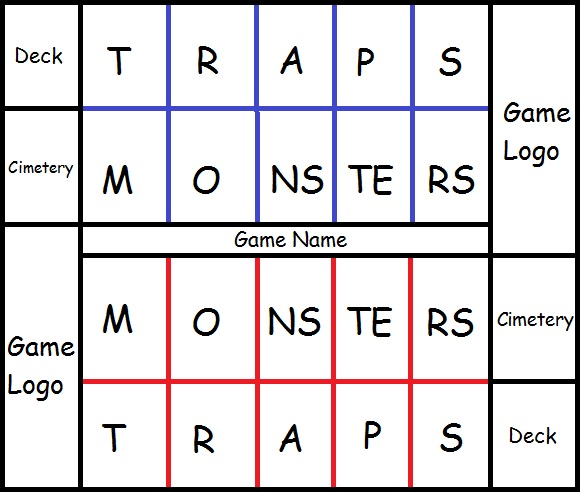
\includegraphics{E:/Documents/Github/Klifehrian/Specifications/gameboardcard.jpg}
	\caption{Schema of the game board}
	\label{fig:gameboardcard}
\end{figure}

%-------------------------------------------------------------------------------------------
%-------------------------------------------------------------------------------------------
%-------------------------------------------------------------------------------------------
\part{Music}
\chapter{What do we feel the player?}
Klifehrian original themes composition was started circa february 2007. At this time, the project was developed on RPG MAKER platform, which only supports Audio or General MIDI loop tracks. So, original Klifehrian soundtrack was originally projected as GM sequences, and a few moment later, as audio tracks (made from MIDI sequences rendered on custom-programmed professional synthesizers).
\\ \\
Now, 7 years later, the big challenges are the following :
\begin{itemize}
\item Organize musical themes by reanalyzing original MIDI sequences.
\item Write some additional themes
\item Think about the ways for dynamically embedding audio segments into the game.
\item Arrange, record, mix those elements.
\end{itemize}
Main musical axes written in 2007 are the following :
\begin{itemize}
\item Klifehrian melody
\item Kren'd\^ur Theme
\item Rufio Theme
\item Ending Bonus Song
\end{itemize}
\newpage Beside this, there were several musics which were associated with events \/ functions :
\begin{itemize}
\item 4 battle themes (2 really used)
\item 3 spooky \/ horror themes
\item victory \/ fail musics
\item Character Theme spin-offs used as event music.
\end{itemize}
\end{document}